\subsection{Speed of loop invariants}
The recommended tactic to solve invariants and ENTAIL goals in VST is \textit{entailer!}. However, we observed that our invariants contained a significiant number of mathematical statements, encoded by VST as PROPs, that were difficult to solve with VST's \textit{entailer!} tactic. As a result, \textit{entailer!} often took a long time to solve or reduce the invariant. To overcome this, we had to pre-solve every PROP in the invariant and preformat the SEP clauses. In the most significant case, an \textit{entailer!} call that took 446 seconds and still returned a large number of unsolved PROPs, was reduced to 36 seconds at the fastest recorded. (Tested on a VirtualBox Lubuntu 18.04 machine assigned 8GB RAM and 2 processors)
\newline\newline
That the tactic could not solve many of our invariant \texttt{PROP}s by itself was expected and reasonable, as they were often complex properties of graphs. However, we were surprised that several solved \texttt{PROP}s took a significant amount of time despite being trivial at first glance. This is especially noticed in PROPs with preconditions of elements in empty lists. Thus, an immediate suggestion to the \textit{entailer!} tactic is to test "\textit{try contradiction}" as early as possible.
\begin{lstlisting}
assert (Hinv_10: forall u v : V,
	In u (nil (A:=V)) -> In v (nil (A:=V)) ->
	connected g u v <-> connected edgeless_graph' u v). {
		intros. contradiction.
}
\end{lstlisting}
The above Coq assertion in our loop precondition, which was easily solved by two basic tactics, cost an additional 50s when left to \textit{entailer!} to prove.
\newline\newline
Given the possibility that invariants carry PROPs on abstract graph properties that we do not expect \textit{entailer!} to solve, a thought is to provide a reduced version of \textit{entailer!} that does not reason about PROPs at all, but leaves them to the user to solve, and focuses on more VST-specific issues such as SEP and LOCAL clauses. This will be useful for verification of functions that implement abstract models.
\subsection{Modularity of library and VST verification}
In previous work by both VST and our team, the C functions and algorithms we have implemented and verified are isolated with little to no dependency on each other. Even the garbage collector verified by Wang et al was its own, independent of the other verified code in the library. This work is the first step our team has taken in verifying code that uses \textit{previously} verified C code, as discussed in Section 4. While a structure of the CertiGraph library has been explained in Section 1, verified functions and programs by both VST and Wang et al are largely isolated and difficult to re-use - even the garbage collector with complex functions is its own isolated system. We found it a necessity to further re-organise the internal hierarchies in our library, for better modularity and re-use of verified code. We have worked to improve this by providing a clearer separation between mathematical lemmas, VST specifications and proofs.
\newline\newline
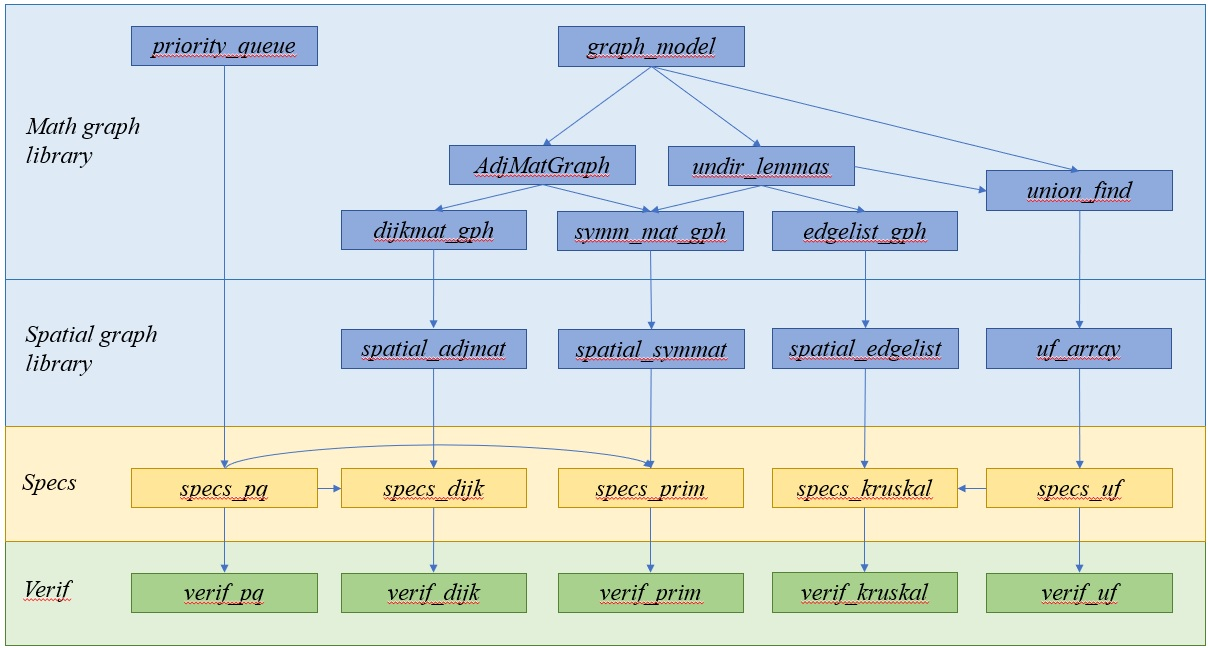
\includegraphics[scale=0.56]{structure.jpg}
\begin{center}Simplified subset of the dependencies in Dijkstra's, Prim's and Kruskal's verification
\end{center}
Previously, we described CertiGraph as having three layers: The mathematical layer which contains "pure Coq" mathematical models and lemmas; the spatial layer to represent graphs in Verifiable C; and the verification layer, for specifications and verifications of C code, whose ASTs were retrieved from CompCert's \textit{clightgen} utility. We further separate this third layer into specifications and verifications. This allows re-use of a previous specification by another system without being burdened by the verification, as illustrated above. The development and verification of components can then be performed in parallel.
\newline\newline
In addition, we have worked to improve on the modularity of the mathematical layer. While we have highlighted differences between directed and undirected graphs, as well as in the graphs in different representations, we have worked to ensure that the same lemmas can be used by them with little need for repetition, to reduce the code base in CertiGraph. Our new contributions to CertiGraph include: ~2000 lines of lemmas of undirected graph properties; ~200 lines to link unionfind properties with undirected graph properties; ~1500 lines for the symmetric matrix graph and ~900 lines for the edgelist graph; ~1800 lines for the verification of Prim's and Kruskal's algorithms each.
\newline\newline
We illustrate this to highlight the potential of VST for verifying larger, complex programs with modular components.
\iffalse
\paragraph{Shared clightgen issue with libraries.} It is obvious that one must include the dependencies of the program when compiling C code. However, we observe an issue of the opposite nature in VST and CompCert - that when running \textit{clightgen} for a program, one must include all programs that \textit{use} the same dependency to properly regenerate the AST files. Failure to do so results in the other program failing to run due to the dependency's changed AST file.
\newline\newline
For instance, in the above figure, both Dijkstra's and Prim's implementations are dependent on the priority queue. When running clightgen for Prim's, we include the priority queue's C implementation to regenerate the AST tree. However, without including Dijkstra's in the same command, the verification of Dijkstra's will result in an error over priority queue's new AST tree.
\newline\newline
(ok this may not be relevant anymore now that we're operating on two different pqs)
\newline\newline
This is a hindrance to the modular design we aspire to, and is thus worth looking into. As of the writing of this paper, we have not looked into the exact nature of the AST files to suggest a solution to VST and CompCert.
\fi